\documentclass{beamer}
\usetheme{Malmoe}

\usepackage{graphicx}
\usepackage{minted}

\usepackage{tikz}
\usetikzlibrary{positioning,shapes,shadows,arrows}
\tikzstyle{object}=[rectangle, draw=black, rounded corners, fill=blue!40, drop shadow,
        text centered, anchor=north, text=white, text width=3cm]
\tikzstyle{highlight}=[rectangle, draw=black, rounded corners, fill=red!40, drop shadow,
        text centered, anchor=north, text=white, text width=3cm]

\tikzstyle{comment}=[rectangle, draw=black, rounded corners, fill=white, drop shadow,
        text centered, anchor=north, text=black, text width=3cm]

\title{From 0 to DIY Web App in 120 minutes}
\author[daniel@axtens.net]{Daniel Axtens\\daniel@axtens.net\\@daxtens}

\setbeameroption{show notes}

\begin{document}

% -------------------------------------------
\begin{frame}[plain]
  \titlepage
\end{frame}


\begin{frame}
  \frametitle{Outline}
  \tableofcontents
\end{frame}

% -------------------------------------------

\section{Getting Started}

\begin{frame}
  \frametitle{Start thinking...}
  \begin{itemize}
  \item There's no set end product for this workshop. There will be
    several spots where you can decide for yourself what to do, and
    assistance in making it happen.

  \item Start thinking about a (relatively) simple application that
    reads from \textbf{and} writes to a free-form-ish database. Perhaps:
    \begin{itemize}
    \item Collate information from a variety of internet-connected
      sensors, process it, and display a
      result. (e.g. average/min/max?)
    \item A database of quotable quotes, with up/down-voting
    \item Configurable Insult/3 word slogan/etc
      generator
    \item Your idea here.
    \item Really stuck? (Yet another) blog with comments, photo-sharing service,
      todo list, calendar, social-bookmarking service, etc. (Most of
      these things are better built with e.g. Django)
    \end{itemize}
  \end{itemize}
\end{frame}

\begin{frame}
  \frametitle{Get on the internet}
  \begin{itemize}
  \item Get on the internet.

  \item Go to \textbf{TODO: URL HERE} to get these instructions so you
    can follow along at your own pace!
  \end{itemize}
\end{frame}


\begin{frame}
  \frametitle{Local environment}
  \begin{itemize}
  \item Set up git to point this to your repository, not mine.
    \begin{itemize}
    \item Fork the repo on GitHub.
    \item \texttt{git remote set-url origin git@github.com:\textit{YOU}/diy-web-app.git}
    \end{itemize}
  \item \texttt{vagrant up}
  \item \texttt{vagrant ssh}
  \item Any changes you make to your local file system are reflected in the virtual machine in the \texttt{/vagrant} directory.
  \item Open another terminal tab for the next step.
  \end{itemize}
\end{frame}

\begin{frame}
  \frametitle{Remote environment}
  
  \begin{itemize}
  \item You get a week of AWS time to build/experiment with your app.
  \item AWS (Amazon Web Services) $\to$ a set of services.
    \begin{itemize}
    \item EC2 - Elastic Cloud Compute $\to$ Virtual Machines
    \item SES - Simple Email Service
    \item Route 53 - DNS service $\to$ maps names like google.com to
      IP addresses like 203.8.182.219
    \item S3 - Simple Storage Service $\to$ Way to store static assets/files.
    \item CloudFront - CDN (Content Delivery Network) $\to$ caches
      static assets near the user for faster speed, less load on your
      server.
    \item And many, many more.
    \end{itemize}
  \item Not free in general, but a free tier exists.
  \end{itemize}
\end{frame}

\begin{frame}
  \frametitle{Remote Environment}
  \begin{itemize}
  \item You should have a bit of paper with the details of your EC2
    instance.
  \item Download the key file.
  \item Use it to log in to the \texttt{ubuntu} user. \\
    \texttt{ssh-add \textit{path-to-your-key-file}} \\
    \texttt{ssh ubuntu@\textit{your-host-name}}
  \item Update the package lists and packages: \texttt{sudo apt-get
      update; sudo apt-get upgrade; sudo reboot}
  \end{itemize}
\end{frame}

\section{Anatomy of a simple web app}

\subsection{Overview}

\begin{frame}
  \frametitle{Anatomy of a simple web app: overview}

  \begin{center}
    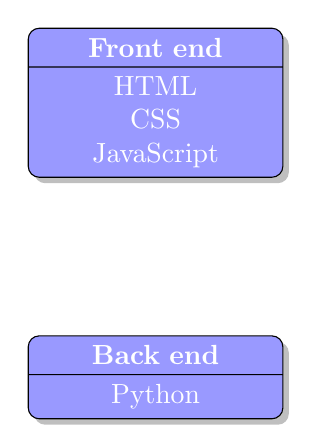
\begin{tikzpicture}[node distance=2cm]
      \node (Frontend) [object, rectangle split, rectangle split parts=2]
      {
        \textbf{Front end}
        \nodepart{second}HTML \\ CSS \\ JavaScript
      };
      \node (Backend) [object, rectangle split, rectangle split parts=2, below=of Frontend]
      {
        \textbf{Back end}
        \nodepart{second}Python
      };
    \end{tikzpicture}
  \end{center}
\end{frame} 

\begin{frame}
  \frametitle{Anatomy of a simple web app: now add a database}
  \begin{center}
      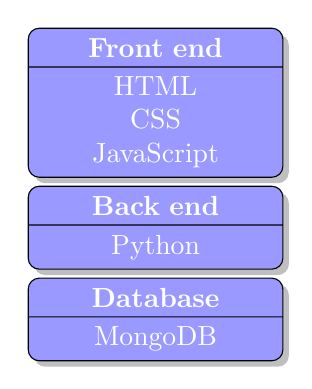
\begin{tikzpicture}[node distance=2cm]
        \node (Frontend) [object, rectangle split, rectangle split parts=2]
        {
          \textbf{Front end}
          \nodepart{second}HTML \\ CSS \\ JavaScript
        };
        \node (Backend) [object, rectangle split, rectangle split parts=2, below=0.1cm of Frontend]
        {
          \textbf{Back end}
          \nodepart{second}Python
        };
        \node (Database) [object, rectangle split, rectangle split parts=2, below=0.1cm of Backend]
        {
          \textbf{Database}
          \nodepart{second}MongoDB
        };
      \end{tikzpicture}
    \end{center}
\end{frame}

\subsection{Delivery}

\begin{frame}
  \frametitle{Anatomy of a simple web app: how does this get to you?}
  \framesubtitle{Ideal world}
  \begin{center}
      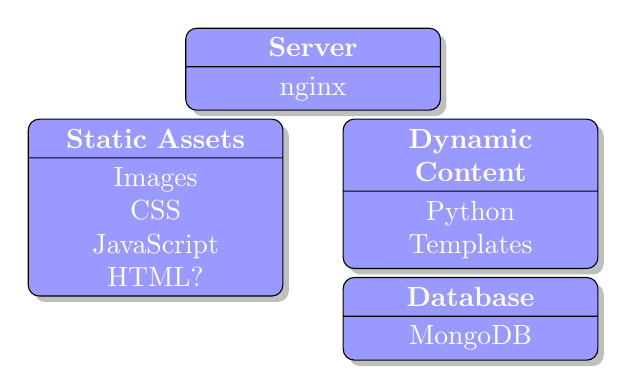
\begin{tikzpicture}[node distance=0.1cm]
        \node (Server) [object, rectangle split, rectangle split parts=2]
        {
          \textbf{Server}
          \nodepart{second}nginx
        };
        \node (Frontend) [object, rectangle split, rectangle split parts=2, below=of Server, xshift=-2cm]
        {
          \textbf{Static Assets}
          \nodepart{second}Images \\ CSS \\ JavaScript \\HTML?
        };
        \node (Backend) [object, rectangle split, rectangle split parts=2, below=of Server, xshift = 2cm]
        {
          \textbf{Dynamic Content}
          \nodepart{second}Python\\Templates
        };
        \node (Database) [object, rectangle split, rectangle split parts=2, below=of Backend]
        {
          \textbf{Database}
          \nodepart{second}MongoDB
        };
      \end{tikzpicture}
    \end{center}
\end{frame}

\begin{frame}
  \frametitle{Anatomy of a simple web app: how does this get to you?}
  \framesubtitle{Our world}
  \begin{center}
      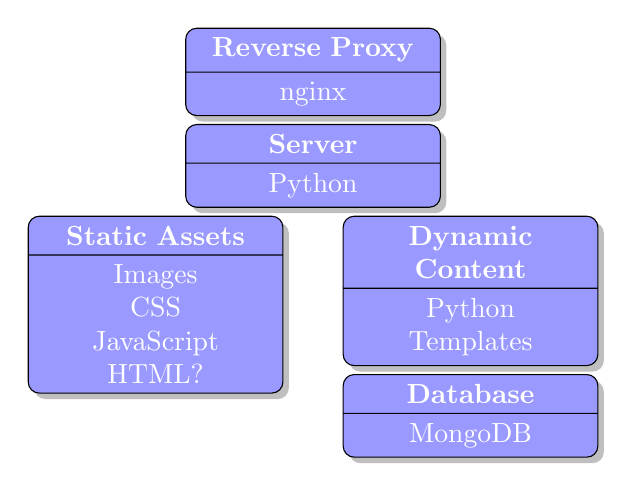
\begin{tikzpicture}[node distance=0.1cm]
        \node (proxy) [object, rectangle split, rectangle split parts=2]
        {
          \textbf{Reverse Proxy}
          \nodepart{second}nginx
        };
        \node (Server) [object, rectangle split, rectangle split parts=2, below=of proxy]
        {
          \textbf{Server}
          \nodepart{second}Python
        };
        \node (Frontend) [object, rectangle split, rectangle split parts=2, below=of Server, xshift=-2cm]
        {
          \textbf{Static Assets}
          \nodepart{second}Images \\ CSS \\ JavaScript \\ HTML?
        };
        \node (Backend) [object, rectangle split, rectangle split parts=2, below=of Server, xshift = 2cm]
        {
          \textbf{Dynamic Content}
          \nodepart{second}Python\\Templates
        };
        \node (Database) [object, rectangle split, rectangle split parts=2, below=of Backend]
        {
          \textbf{Database}
          \nodepart{second}MongoDB
        };
      \end{tikzpicture}
    \end{center}
\end{frame}

\section{Building your app}

\begin{frame}
  \frametitle{Building your app}
\end{frame}

\subsection{Server}

\begin{frame}
  \frametitle{Server}
    \begin{center}
      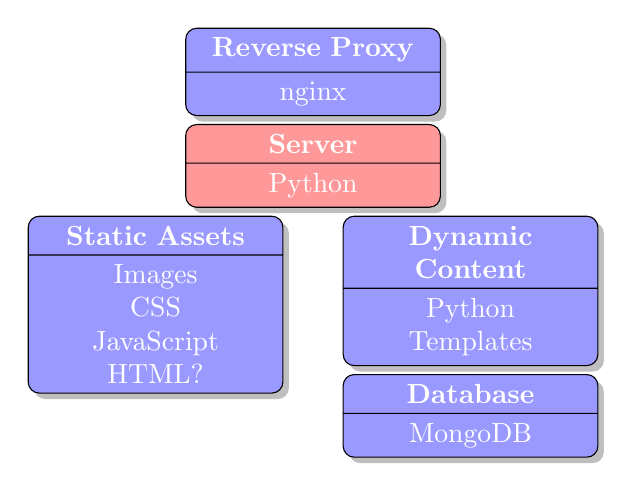
\begin{tikzpicture}[node distance=0.1cm]
        \node (proxy) [object, rectangle split, rectangle split parts=2]
        {
          \textbf{Reverse Proxy}
          \nodepart{second}nginx
        };
        \node (Server) [highlight, rectangle split, rectangle split parts=2, below=of proxy]
        {
          \textbf{Server}
          \nodepart{second}Python
        };
        \node (Frontend) [object, rectangle split, rectangle split parts=2, below=of Server, xshift=-2cm]
        {
          \textbf{Static Assets}
          \nodepart{second}Images \\ CSS \\ JavaScript \\ HTML?
        };
        \node (Backend) [object, rectangle split, rectangle split parts=2, below=of Server, xshift = 2cm]
        {
          \textbf{Dynamic Content}
          \nodepart{second}Python\\Templates
        };
        \node (Database) [object, rectangle split, rectangle split parts=2, below=of Backend]
        {
          \textbf{Database}
          \nodepart{second}MongoDB
        };
      \end{tikzpicture}
    \end{center}
\end{frame}

\begin{frame}
  \frametitle{Introducing Bottle}
  \begin{figure}[h!]
    \centering
    
\includegraphics{imgs/bottle_logo}
    \caption{Bottle is a fast, simple and lightweight WSGI micro web-framework for Python. \url{http://bottlepy.org/}}
    \label{fig:bottle_logo}
  \end{figure}

  You might also want to consider Flask: \url{http://flask.pocoo.org/}. It does a bit more for you/has a bit more magic than Bottle.

\end{frame}

\begin{frame}
  \frametitle{Hello World!}
  Edit \texttt{webapp.py}.
\hrule
  \inputminted{python}{../steps/01-hello-world/01-webapp.py}
\hrule
In your vagrant shell, \texttt{cd /vagrant; python webapp.py}.

Then visit \url{http://localhost:8080} in your browser.
\end{frame}

\begin{frame}
\frametitle{Best practices: commit your changes!}
\texttt{git add webapp.py}\\
\texttt{git commit -m"Hello world example"}\\
\texttt{git push}
\end{frame}

\begin{frame}[fragile]
  \frametitle{Greeting others}
  Let's extend:
  \begin{minted}{python}
@route('/greet/<name>')
def greet(name):
    return "Hello, %s!" % name
  \end{minted}

  \hrule
  \texttt{git add webapp.py}\\
  \texttt{git commit -m"Add greet function"}\\
  \texttt{git push}
\end{frame}

\begin{frame}
  \frametitle{Danger, Will Robinson!}
  Spot the subtle error and potential security hole.

  First to spot it gets a free freddo. TODO CONFIRM
\end{frame}

\begin{frame}
  \frametitle{Danger, Will Robinson!}

  What happens if you go to \url{localhost:8080/greet/<b>Daniel}?

  \textbf{This unescaped HTML has the potential (in other
    circumstances) to cause XSS vulnerabilites.}

  Fortunately, it's easy to avoid.
\end{frame}

\begin{frame}[fragile]
  \frametitle{Safe user input the right way}
  
  {\large Don't try to sanitise it yourself.}

  You will probably miss an edge case.

  \vskip1em

  {\Large Use templates.}

  \begin{minted}{python}
    from bottle import route, run, template

    ...

    def greet(name):
    	return template("Hello, {{name}}!", name=name)
  \end{minted}

\end{frame}

\begin{frame}[fragile]
  \frametitle{Separating presentation and content}
  We don't want template code in \texttt{.py} files.

  Edit \texttt{views/hello.tpl}. Fill it with standard HTML, with
  \texttt{\{\{name\}\}} somewhere. (Lazy? See the link to the sample
  on the notes.)

  Then:
  \begin{minted}{python}
    from bottle import route, run, template, view

    ...

    @route('/greet/<name>')
    @view('hello')
    def greet(name):
    	return {'name': name}
  \end{minted}

  \textbf{Bottle's template language (SimpleTemplate Engine) has more
    features, which we'll cover later...}
\end{frame}

\begin{frame}[fragile]
  \frametitle{Simplifying things}
  Why do we have different functions for \texttt{/} and \texttt{/greet}, when they do
  mostly the same thing? \textbf{A bottle function can handle multiple
  routes.}

  \begin{minted}{python}
@route('/')
@route('/greet/<name>')
@view('hello')
def greet(name="World"):
  \end{minted}
\end{frame}

\begin{frame}
\frametitle{Best practices: commit your changes!}
\texttt{git add webapp.py views/hello.tpl}\\
\texttt{git commit -m"Serve Hello World with a template."}\\
\texttt{git push}
\end{frame}


\begin{frame}[fragile]
  \frametitle{Serving static files}
  \textcolor{red}{\large Put them in a separate sub-directory!}

  \begin{minted}{python}
from bottle import route, run, template, view, static_file
import os

root = os.path.dirname(__file__)
static_root = os.path.join(root, "static")

...

@route('/static/<path:path>')
def static(path):
    return static_file(path, root=static_root)
    \end{minted}
\end{frame}

\begin{frame}
\frametitle{Best practices: commit your changes!}
\texttt{git add webapp.py}\\
\texttt{git commit -m"Serve static files out of static/"}\\
\texttt{git push}
\end{frame}

\begin{frame}
  \frametitle{Server}
    \begin{center}
      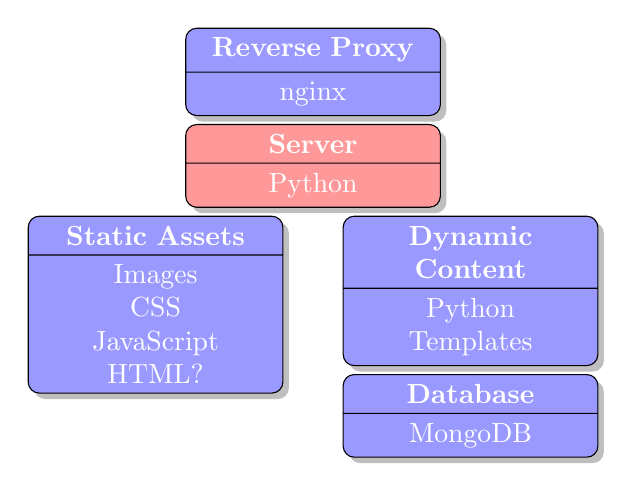
\begin{tikzpicture}[node distance=0.1cm]
        \node (proxy) [object, rectangle split, rectangle split parts=2]
        {
          \textbf{Reverse Proxy}
          \nodepart{second}nginx
        };
        \node (Server) [highlight, rectangle split, rectangle split parts=2, below=of proxy]
        {
          \textbf{Server}
          \nodepart{second}Python
        };
        \node (Frontend) [object, rectangle split, rectangle split parts=2, below=of Server, xshift=-2cm]
        {
          \textbf{Static Assets}
          \nodepart{second}Images \\ CSS \\ JavaScript \\ HTML?
        };
        \node (Backend) [object, rectangle split, rectangle split parts=2, below=of Server, xshift = 2cm]
        {
          \textbf{Dynamic Content}
          \nodepart{second}Python\\Templates
        };
        \node (Database) [object, rectangle split, rectangle split parts=2, below=of Backend]
        {
          \textbf{Database}
          \nodepart{second}MongoDB
        };
      \end{tikzpicture}
    \end{center}
\end{frame}

\subsection{Front end}

\begin{frame}
  \frametitle{Front end}
    \begin{center}
      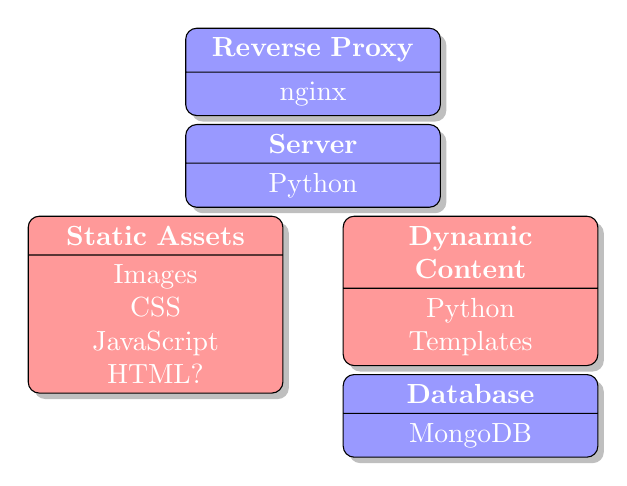
\begin{tikzpicture}[node distance=0.1cm]
        \node (proxy) [object, rectangle split, rectangle split parts=2]
        {
          \textbf{Reverse Proxy}
          \nodepart{second}nginx
        };
        \node (Server) [object, rectangle split, rectangle split parts=2, below=of proxy]
        {
          \textbf{Server}
          \nodepart{second}Python
        };
        \node (Frontend) [highlight, rectangle split, rectangle split parts=2, below=of Server, xshift=-2cm]
        {
          \textbf{Static Assets}
          \nodepart{second}Images \\ CSS \\ JavaScript \\ HTML?
        };
        \node (Backend) [highlight, rectangle split, rectangle split parts=2, below=of Server, xshift = 2cm]
        {
          \textbf{Dynamic Content}
          \nodepart{second}Python\\Templates
        };
        \node (Database) [object, rectangle split, rectangle split parts=2, below=of Backend]
        {
          \textbf{Database}
          \nodepart{second}MongoDB
        };
      \end{tikzpicture}
    \end{center}
\end{frame}

\begin{frame}
  \frametitle{Introducing Bootstrap}
  \begin{figure}[h!]
    \centering
    
\includegraphics[scale=0.3]{imgs/bootstrap_banner.png}
    \caption{Bootstrap: \url{getbootstrap.com}}
    \label{fig:bootstrap_banner}
  \end{figure}

  \begin{itemize}
  \item We're lazy, so we use Bootstrap for the frontend.
\end{itemize}
\end{frame}

\begin{frame}[fragile]
\frametitle{Setting up Bootstrap}
\begin{itemize}
  \item Download it from \url{getbootstrap.com}, extract the archive,
    put the folders in \texttt{static/}
  \item Choose the example from
    \url{http://getbootstrap.com/getting-started/#examples} that best
    suits your project.
    \begin{itemize}
    \item (Optionally) find it on GitHub.
    \item Copy the code to \texttt{views/index.tpl}
    \item Download any extra stylesheets, etc.
    \item Adjust all links to read \texttt{/static/\{js, css, etc\}/...}
    \end{itemize}
  \item Adjust your code to use the \texttt{index} template, not the
  \texttt{hello} one.
\end{itemize}
\end{frame}

\end{document}
